\documentclass{beamer}
\usetheme{metropolis}
\usepackage{graphicx}
\usepackage{subfig}
\usepackage{tcolorbox}
\title{Calculus-Based Physics-2: Electricity, Magnetism, and Thermodynamics (PHYS180-02): Unit 5}
\author{Jordan Hanson}
\institute{Whittier College Department of Physics and Astronomy}

\begin{document}
\maketitle

\section{Unit 4 Review}

\begin{frame}{Unit 4 Summary}
\textbf{Reading: Chapters 7, 9, and 10}
\begin{enumerate}
\item \alert{Voltage and Capacitance}
\item Ohm's Law
\item DC circuits
\end{enumerate}
\end{frame}

\section{Unit 4 Review Problems}

\begin{frame}{Unit 4 Review Problems}
\begin{columns}[T]
\begin{column}{0.5\textwidth}
Which of the following would decrease the time required to charge the capacitor at right?
\begin{itemize}
\item A: Decreasing the capacitance
\item B: Decreasing the resistance
\item C: It already charges as fast as possible
\item D: Both A and B
\end{itemize}
\end{column}
\begin{column}{0.5\textwidth}
\begin{figure}
\centering
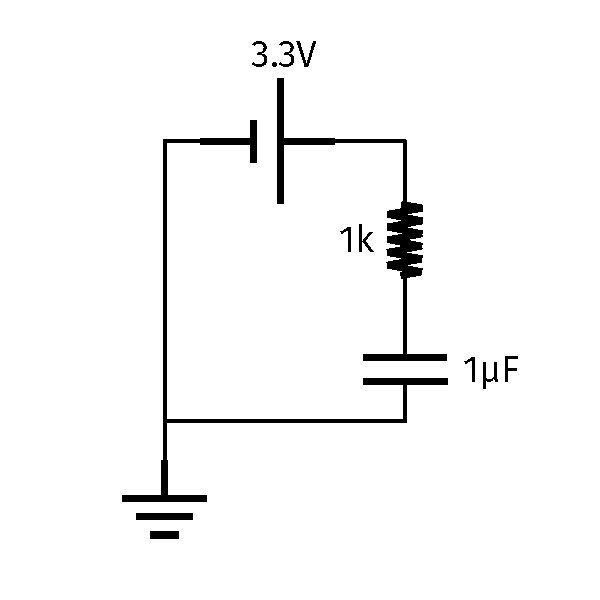
\includegraphics[width=0.8\textwidth]{figures/iVCurve7.pdf}
\caption{\label{fig:RC0} An RC circuit.}
\end{figure}
\end{column}
\end{columns}
\end{frame}

\begin{frame}{Unit 4 Review Problems}
\begin{columns}[T]
\begin{column}{0.5\textwidth}
What is the RC time of the circuit?
\begin{itemize}
\item A: 1 $\mu$s
\item B: 1 ms
\item C: 1 s
\item D: 10 s
\end{itemize}
\end{column}
\begin{column}{0.5\textwidth}
\begin{figure}
\centering
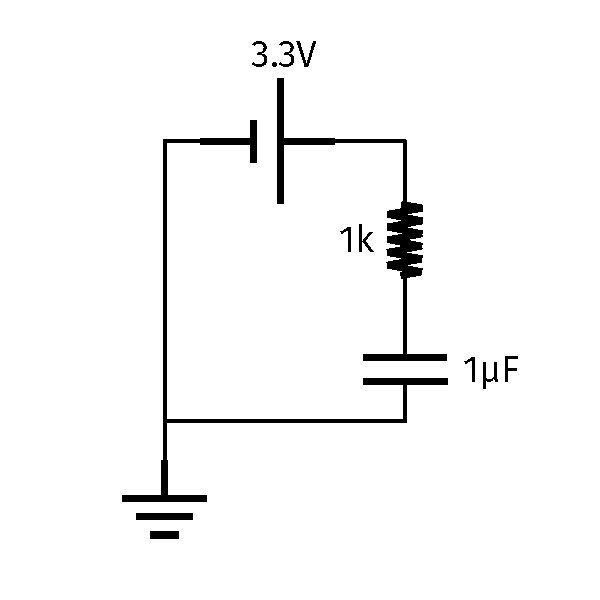
\includegraphics[width=0.8\textwidth]{figures/iVCurve7.pdf}
\caption{\label{fig:RC1} An RC circuit.}
\end{figure}
\end{column}
\end{columns}
\end{frame}

\begin{frame}{Unit 4 Review Problems}
\begin{columns}[T]
\begin{column}{0.5\textwidth}
What is the maximum charge stored eventually in the capacitor?  \textit{Recall that $Q = CV$}.
\begin{itemize}
\item A: 3.3 $\mu$ C
\item B: 1.5 $\mu$ C
\item C: 3.3 mC
\item D: 1.5 C
\end{itemize}
\end{column}
\begin{column}{0.5\textwidth}
\begin{figure}
\centering
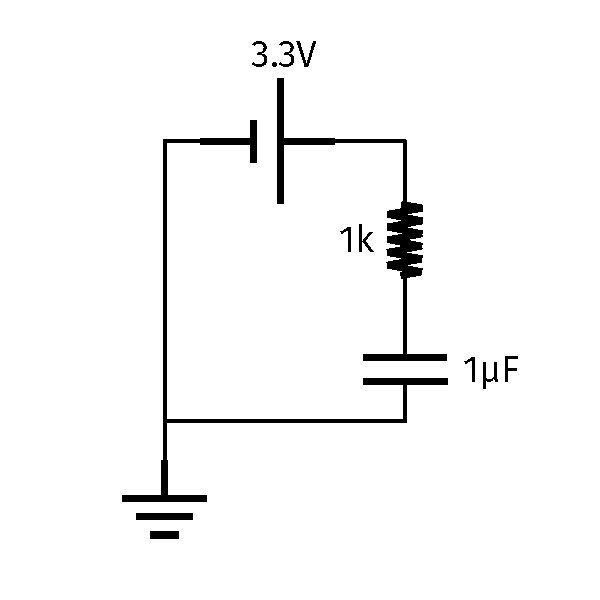
\includegraphics[width=0.8\textwidth]{figures/iVCurve7.pdf}
\caption{\label{fig:RC2} An RC circuit.}
\end{figure}
\end{column}
\end{columns}
\end{frame}

\section{Summary}

\begin{frame}{Unit 5 Summary}
\textbf{Reading: Chapter 11}
\begin{enumerate}
\item Magnetism and magnetic fields
\item \alert{Motion of a charged particle in a magnetic field}
\item Other forces
\item Current loops
\end{enumerate}
\end{frame}

\section{Magnetism and magnetic fields}

\begin{frame}{Magnetism and magnetic fields}
\begin{figure}
\centering
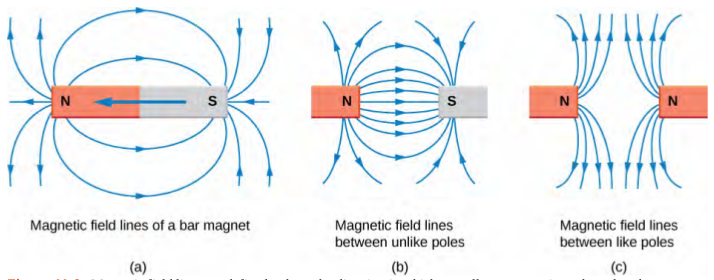
\includegraphics[width=0.9\textwidth,trim=0cm 1cm 0cm 0cm,clip=true]{figures/fields1.png}
\caption{\label{fields1} Various magnetic field line configurations.}
\end{figure}
\end{frame}

\begin{frame}{Magnetism and magnetic fields}
\begin{figure}
\centering
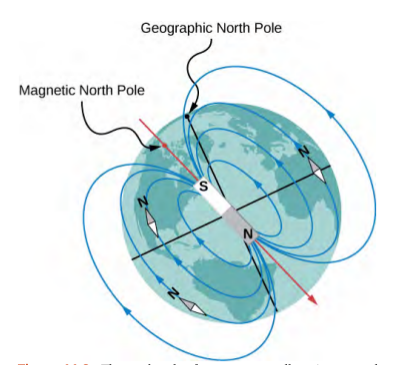
\includegraphics[width=0.6\textwidth,trim=0cm 0.1cm 0cm 0cm,clip=true]{figures/fields2.png}
\caption{\label{fields2} The magnetic and geographic poles are not the same.}
\end{figure}
\end{frame}

\begin{frame}{Magnetism and magnetic fields}
It would be nice if we could say:
\begin{equation}
F = \mu_0 \frac{q_{m,1} g_{m,2}}{r^2}
\end{equation}
But...we can't.  Why?  There's no such thing has magnetic charge:
\begin{align}
\nabla \cdot \vec{E} &= \rho/\epsilon_0 \\ 
\nabla \cdot \vec{B} &= 0
\end{align}
But there is a force associating charge and magnetic fields.  But first, let's review the cross-product.
\end{frame}

\begin{frame}{Magnetism and magnetic fields}
What is a cross-product and how does it work? \\ \vspace{0.25cm}
\begin{figure}
\centering
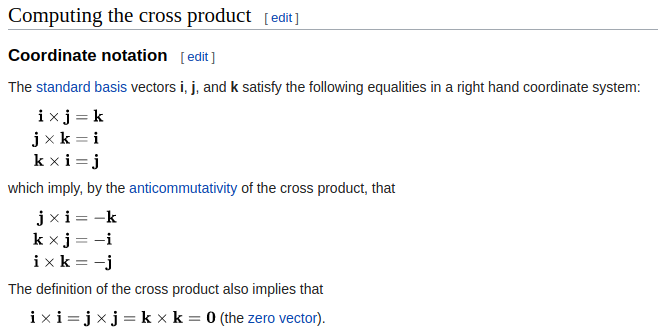
\includegraphics[width=0.75\textwidth]{figures/crossP.png}
\caption{\label{fig:crossP} The cross-product is a way of multiplying unit vectors.}
\end{figure}
\end{frame}

\begin{frame}{Magnetism and magnetic fields}
Let $\vec{v} = 2\hat{i}$ and $w = -2 \hat{j}$.  What is $\vec{v} \times \vec{w}$?
\begin{itemize}
\item A: $-4 \hat{k}$
\item B: $4 \hat{k}$
\item C: $-2 \hat{i}$
\item D: $2 \hat{j}$
\end{itemize}
\end{frame}

\begin{frame}{Magnetism and magnetic fields}
Let $\vec{v} = 3\hat{j}$ and $w = 5 \hat{k}$.  What is $\vec{v} \times \vec{w}$?
\begin{itemize}
\item A: $15 \hat{i}$
\item B: $5 \hat{j}$
\item C: $3 \hat{i}$
\item D: $15 \hat{k}$
\end{itemize}
\end{frame}

\begin{frame}{Magnetism and magnetic fields}
Let $\vec{v} = 3\hat{i} \times 3\hat{j}$ and $w = 2 \hat{k}$.  What is $\vec{v} \times \vec{w}$?
\begin{itemize}
\item A: $-6 \hat{j} + 6\hat{k}$
\item B: $-6 \hat{j} + 6\hat{i}$
\item C: $6 \hat{j} + 6\hat{i}$
\item D: $6 \hat{k} + 6\hat{i}$
\end{itemize}
\end{frame}

\begin{frame}{Magnets and magnetic fields}
\textbf{Group board exercise:} Compute the following cross product:
\begin{align}
\vec{v} &= 2\hat{i}-2\hat{j} \\
\vec{w} &= 4\hat{j}-4\hat{i} \\
\vec{v} \times \vec{w} &= ??
\end{align}
\end{frame}

\begin{frame}{Magnets and magnetic fields}
\textbf{Group board exercise:} Compute the following cross product:
\begin{align}
\vec{v} &= 2\hat{i}-2\hat{j}+\hat{k} \\
\vec{w} &= 4\hat{j}-4\hat{i}-\hat{k} \\
\vec{v} \times \vec{w} &= ??
\end{align}
\end{frame}

\begin{frame}{Magnets and magnetic fields}
\begin{tcolorbox}[colback=white,colframe=red!40!blue,title=The Lorentz Force]
\alert{Let a particle with charge q and velocity $\vec{v}$ move through a magnetic field $\vec{B}$. The Lorentz force on the charged particle is
\begin{equation}
\vec{F}_{\rm L} = q\vec{v} \times \vec{B}
\label{eq:Lorentz}
\end{equation}}
\end{tcolorbox}
\textit{As a helpful memory tool, we have the right-hand rule to
remember the direction of the cross-product.} The units of the
magnetic field are the Telsa, after Nikola Tesla. We also have
the Gauss which is $10^{-4}$ Tesla.
\end{frame}

\begin{frame}{Magnets and magnetic fields}
\begin{figure}
\centering
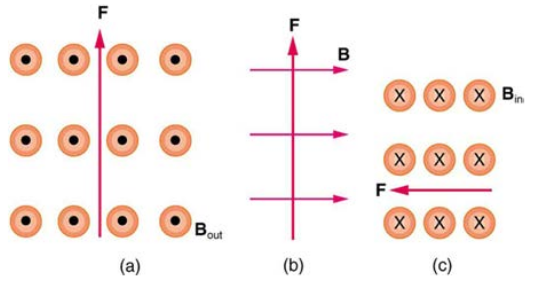
\includegraphics[width=0.75\textwidth]{figures/lorentzProblem.png}
\caption{\label{fig:lorentzProblem} Three different magnetic field and charge scenarios. The
vector $\vec{F}$ is the direction of the Lorentz force, and the magnetic field
is uniform. A dot indicates that the magnetic field is coming out of
the page, and an x indicates that the field is going into the page.}
\end{figure}
\end{frame}

\begin{frame}{Magnets and magnetic fields}
\begin{columns}[T]
\begin{column}{0.3\textwidth}
In which of the diagrams is a positively charged particle moving to the left?
\begin{itemize}
\item A: A
\item B: B
\item C: C
\item D: WAT WAT WAT
\end{itemize}
\end{column}
\begin{column}{0.7\textwidth}
\begin{figure}
\centering
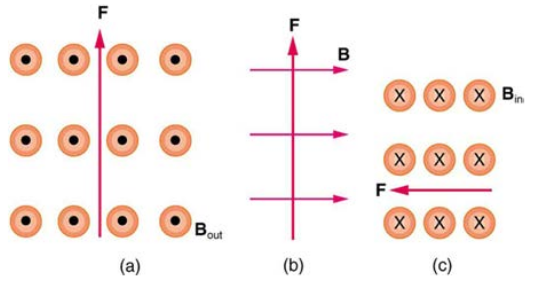
\includegraphics[width=0.75\textwidth]{figures/lorentzProblem.png}
\caption{\label{fig:lorentzProblem2} Three different magnetic field and charge scenarios.}
\end{figure}
\end{column}
\end{columns}
\end{frame}

\begin{frame}{Magnets and magnetic fields}
\begin{columns}[T]
\begin{column}{0.3\textwidth}
In which of the diagrams is a positively charged particle moving upwards?
\begin{itemize}
\item A: A
\item B: B
\item C: C
\item D: WAT WAT WAT
\end{itemize}
\end{column}
\begin{column}{0.7\textwidth}
\begin{figure}
\centering
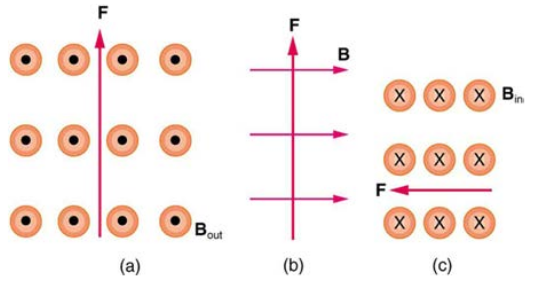
\includegraphics[width=0.75\textwidth]{figures/lorentzProblem.png}
\caption{\label{fig:lorentzProblem3} Three different magnetic field and charge scenarios.}
\end{figure}
\end{column}
\end{columns}
\end{frame}

\begin{frame}{Magnets and magnetic fields}
\begin{columns}[T]
\begin{column}{0.3\textwidth}
In which of the diagrams is a negatively charged particle into the page?
\begin{itemize}
\item A: A
\item B: B
\item C: C
\item D: WAT WAT WAT
\end{itemize}
\end{column}
\begin{column}{0.7\textwidth}
\begin{figure}
\centering
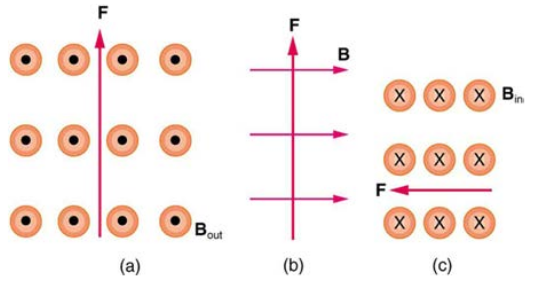
\includegraphics[width=0.75\textwidth]{figures/lorentzProblem.png}
\caption{\label{fig:lorentzProblem4} Three different magnetic field and charge scenarios.}
\end{figure}
\end{column}
\end{columns}
\end{frame}

\begin{frame}{Magnets and magnetic fields}
\begin{columns}[T]
\begin{column}{0.3\textwidth}
In which of the diagrams is a negatively charged particle to the right?
\begin{itemize}
\item A: A
\item B: B
\item C: C
\item D: WAT WAT WAT
\end{itemize}
\end{column}
\begin{column}{0.7\textwidth}
\begin{figure}
\centering
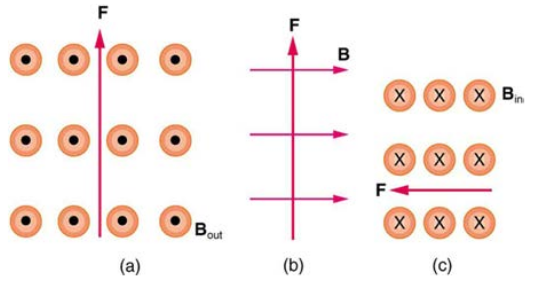
\includegraphics[width=0.75\textwidth]{figures/lorentzProblem.png}
\caption{\label{fig:lorentzProblem5} Three different magnetic field and charge scenarios.}
\end{figure}
\end{column}
\end{columns}
\end{frame}

\begin{frame}{Magnets and magnetic fields}
A theorem for the magnitude of the cross-product:  Let $\vec{a}$ and $\vec{b}$ be vectors and $\theta$ be the angle between them.  The magnitude of the cross product is:
\begin{equation}
|\vec{a} \times \vec{b}| =  a b \sin\theta
\end{equation}
Thus, the magnitude of the Lorentz force is
\begin{equation}
F_{\rm L} = q v B \sin\theta
\end{equation}
The angle $\theta$ is between the velocity and the magnetic field.
\end{frame}

\begin{frame}{Magnets and magnetic fields}
A cosmic ray proton moving toward the Earth at $3 \times 10^{6}$ m/s experiences a magnetic force of $2 \times 10^{-17}$ N. What is the strength of the magnetic field of the Earth? (1 Gauss = $10^{-4}$ Tesla).
\begin{itemize}
\item A: 0.1 Gauss
\item B: 0.6 Gauss
\item C: 1 Gauss
\item D: 6 Gauss
\end{itemize}
\end{frame}

\begin{frame}{Magnets and magnetic fields}
\begin{figure}
\centering
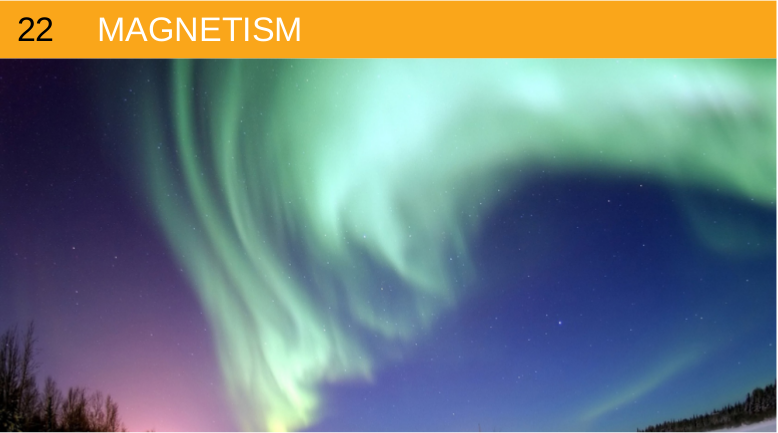
\includegraphics[width=0.9\textwidth]{figures/aurora.png}
\caption{\label{fig:aurora} The aurora borealis, or northern lights.}
\end{figure}
\end{frame}

\begin{frame}{Magnets and magnetic fields}
A cool talk on the aurora borealis:
\url{https://youtu.be/czMh3BnHFHQ} \\
\begin{figure}
\centering
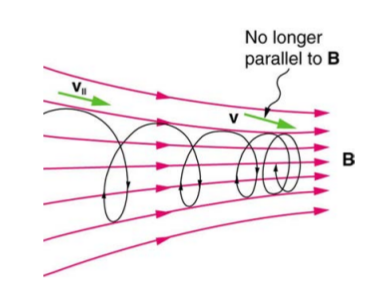
\includegraphics[width=0.45\textwidth]{figures/mag1.png}
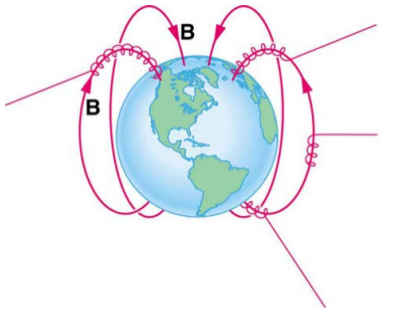
\includegraphics[width=0.45\textwidth]{figures/mag2.png}
\end{figure}
One un-explained piece: what does it mean for the electrons and protons to \textit{high-five} the neutral oxygen and nitrogen atoms?
\end{frame}

\section{Conclusion}

\begin{frame}{Unit 5 Summary}
\textbf{Reading: Chapter 11}
\begin{enumerate}
\item Magnetism and magnetic fields
\item \alert{Motion of a charged particle in a magnetic field}
\item Other forces
\item Current loops
\end{enumerate}
\end{frame}

\section{Answers}

\begin{frame}{Answers}
\tiny
\begin{columns}[T]
\begin{column}{0.5\textwidth}
\begin{itemize}
\item Both A and B
\item 1 ms
\item 3.3 $\mu$ C
\end{itemize}
\end{column}
\begin{column}{0.5\textwidth}
\begin{itemize}
\item 
\end{itemize}
\end{column}
\end{columns}
\end{frame}

\end{document}
